\documentclass{article}
\usepackage{amsmath}
\usepackage{amssymb}
\usepackage{enumerate}
\usepackage{listings}
\usepackage{graphicx}
\usepackage{caption}
\usepackage{subcaption}
\usepackage[T1]{fontenc}
\usepackage{MnSymbol}

\newcommand\vtt[1]{{\normalfont\fontfamily{cmvtt}\selectfont #1}}
\newcommand\independent{\protect\mathpalette{\protect\independenT}{\perp}}
\def\independenT#1#2{\mathrel{\rlap{$#1#2$}\mkern2mu{#1#2}}}

\def\ci{\perp\!\!\!\perp}

\begin{document}
\title{Homework 4 - Final Writeup}
\author{Patrick Collins}
\date{\today}
\maketitle

\section{Writeup}

\begin{enumerate}[(a)]

\item Imagine that some node $y_m$ is missing.

\begin{itemize}
\item How does this change the definition of $\alpha_t(i)$ and $\beta_t(i)$?

It does not change the definition of $\alpha_t(i)$ or $\beta_t(i)$ --- $y_m$
can simply be kept in the model as a hidden node and both formulae can
remain unchanged.

\item Derive a formula for $p(y_m | y_0,\dots, y_{m-1},
  y_{m+1},\dots,y_T)$.

First, note that $p(y_m | y_0,\dots, y_{m-1},
  y_{m+1},\dots,y_T) = p(y_m | y_0,\dots, y_{m-1})  p(y_m | y_{m-1},\dots, y_T)$


Noting that the HMM is a directed graphical model, in this case, $y_m$
will be determined entirely by the value of the corresponding hidden
node (which I will call $x_m$) attached to it. The probability that
$y_m$ takes on some particular value $j$, therefore, is expressed by
the probability that $x_m$ emits $j$. The whole expression is given by
(letting $Y = y_0,\dots, y_{m-1}, y_{m+1}, y_T$ for brevity):

\begin{align*}
p(y_m = j |Y) &= \sum \limits_{i=1}^{N_h} p(x_m = i |Y) \omega_{i, j}\\
&= \sum \limits_{i=1}^{N_h} \gamma_t(i)  \omega_{i, j}
\end{align*}
\end{itemize}

Hence we find the most likely assignment to $y_m$, $\hat{y}_m$ by
finding:
\begin{equation*}
\hat{y}_m = \arg\!\max_j(\sum \limits_{i=1}^{N_h} \gamma_t(i)  \omega_{i, j})
\end{equation*}

\item Prove $p(x_t|y_0,\dots,y_T) = \frac {\alpha_t(x_t)\beta_t(x_t)}
  {\sum_{x_t'}\alpha'_t(x'_t)\beta_t(x'_t)}p(x_{t+1}|x_t)p(y_{t+1} | x_{t+1})$

First, apply Bayes rule and cancel terms (based on our assumptions of
statistical independence --- namely that no $y_i$ depends on any other
$y_j$, and no $x_i$ depends on any other $x_j$:

\begin{align*}
p(x_t, x_{t+1} | y_0,\dots,y_T) &= p(y_{t+2},\dots,y_T | x_{t+1})p(y_0, \dots, y_{t+1}, x_{t+1}, x_t)\\
&= p(y_{t+2},\dots,y_T | x_{t+1})p(y_{t+1} | x_{t+1}) p(y_0, \dots, y_t, x_{t+1}, x_t)\\
&= p(y_{t+2},\dots,y_T | x_{t+1})p(y_{t+1} | x_{t+1}) p(x_{t+1} | x_t) p(y_0, \dots, y_{t} | x_t)\\
&= \alpha_t(x_t) \beta_{t+1}(x_{t+1}) p(y_{t+1} | x_{t+1}) p (x_{t+1}, x_t)\\
\end{align*}

Then multiply by $\beta(x_t) / \beta(x_t)$ and normalize (following the
directions on slide 15 of the Hidden Markov Model lecture) by a factor
of $\sum \limits_{x'_t} \alpha_t(x'_t)\beta_t(x'_t)$ to yield:

\begin{align*}
  \alpha_t(x_t) \beta_{t+1}(x_{t+1}) p(y_{t+1} | x_{t+1}) p(x_{t+1}, x_t) &= \frac {\alpha_t(x_t) \beta_t(x_t) \beta(x_{t+1}) p(y_{t+1} | x_{t+1}) p (x_{t+1}, x_t)} {\beta_t(x_t) \sum \limits_{x'_t} \alpha_t(x'_t)\beta_t(x'_t)}\\
  \alpha_t(x_t) \beta_{t+1}(x_{t+1}) p(y_{t+1} | x_{t+1}) p(x_{t+1}, x_t) &= \frac {\gamma_t(x_t) \beta_t(x_{t +1})} {\beta_t(x_t)} p(y_{t+1} | x_{t+1}) p(x_{t+1}, x_t)
\end{align*}

which is what we wanted to show.


\item Express the log likelihood of each term, prove that they are
  maximized with the given operation, and explain the intuitive
  meaning of each term.


Beginning with the initial expression, we distribute the outer
summation and the $p(x_0\dots,x_T | y_0,\dots,y_T)$ term:

\begin{align*}
\mathbb{E}(\log l(\pi, \theta, \omega)) &= \sum \limits_{x_0\dots,x_T}\left[\log\pi_{x_0} + \sum_{t=1}^T \log\theta_{x_{t-1}, x_t} + \sum_{t=1}^T\log\omega_{x_T,y_t}\right]p(x_0\dots,x_T | y_0,\dots,y_T)&\\
\mathbb{E}(\log l(\pi, \theta, \omega)) &= \sum \limits_{x_0\dots,x_T} (\log\pi_{x_0})p(x_0\dots,x_T | y_0,\dots,y_T) +&\\
&\sum \limits_{x_0\dots,x_T}  (\sum_{t=1}^T \log\theta_{x_{t-1}, x_t})p(x_0\dots,x_T | y_0,\dots,y_T) + &\\
&\sum \limits_{x_0\dots,x_T} (\sum_{t=1}^T\log\omega_{x_T,y_t})p(x_0\dots,x_T | y_0,\dots,y_T)&\\
\end{align*}

and now consider each one independently.

Noting the assumptions of independence for HMM (namely that $p(x_{t})
\independent  p(x_{t'}) | p(x_{t-1})$) the first term simplifies:
\begin{align*}
 \sum \limits_{x_0\dots,x_T} \log\pi_{x_0}p(x_0\dots,x_T | y_0,\dots,y_T) &=  \sum_{i=0}^h \pi_{x_i} p(x_i | y_0\dots y_T)\\
&= \sum_{i=0}^{N_h} \log\pi_{x_i}\gamma_0(i)
\end{align*}

To minimize this expression, we take the derivative with respect to
$\pi_i$, constrain $\pi$ such that $\sum_i\pi_i = 1$ (since it represents a
distribution) and add a Lagrange multiplier $\lambda$, we get:

\begin{equation*}
\frac \partial {\partial\pi_{x_i}} \left(\sum_{i=0}^h \log\pi_{x_i}\gamma_0(i) +
  \lambda(\sum_{i=0}^h\pi_{x_i} - 1) \right)  = 0
\end{equation*}

and, taking the derivative, summing over $i$ to get $\lambda$, we arrive at
an optimum value for $\pi^{\text{new}}_i$ of

\begin{equation*}
\pi^{\text{new}}_i = \gamma_0(i)
\end{equation*}

which is what we wanted to show. Intuitively, this represents setting
the likelihood that the HMM begins at $t = 0$ in state $i$ to the
expected number of times that the HMM is in state $i$ at $t = 0$.

Beginning with the next expression, noting again the assumptions of
independence, we have

\begin{align*}
\sum_{x_0\dots,x_T}  (\sum_{t=1}^T \log\theta_{x_{t-1}, x_t})&p(x_0\dots,x_T | y_0,\dots,y_T)\\
&= \sum_{x_0\dots,x_T} \sum_{i=1}^{N_h} \sum_{j=1}^{N_h} (\log\theta_{i, j})p(x_t = i, x_{t+1} = j | y_0 \dots y_T) \\
 &=\sum_{t=1}^{T-1} \sum_{i=1}^{N_h} \sum_{j=1}^{N_h} (\log\theta_{i, j})\xi_t(i, j)
\end{align*}

i.e. here, we are summing the probability of all transitions from $i$
to $j$ for each time $t$. We constrain $\sum_{j=1}^{N_h}\theta_{i, j} = 1$,
and, similar to the above, arrive at:

\begin{equation*}
\frac \partial {\partial\theta_{i, j}} \left( \sum_{t=1}^{T-1} \sum_{i=1}^{N_h} \sum_{j=1}^{N_h} (\log\theta_{i, j})\xi_t(i, j) + \lambda(\sum_{j=1}^{N_h}\theta_{i, j} -  1) \right) = 0
\end{equation*}

taking partial derivatives rearranging to solve for $\theta_{i, j}$, we
get:

\begin{align*}
\theta_{i, j} &= \frac {\sum_{t=1}^{T-1} \xi_t(i, j)}{\sum_{t=1}^{T-1} \sum_{j=1}^{N_h} \xi_t(i, j)}\\
&= \frac {\sum_{t=1}^{T-1} \xi_t(i, j)}{\sum_{t=1}^{T-1} \gamma_t(i)}
\end{align*}

which is what we wanted to show. Intuitively this represents setting
the likelihood that the HMM transitions to state $j$ from state $i$ to
the expected number of transitions from $i$ to $j$ divided by the
number of transitions to $j$ over the course of the input just
processed.

Finally, for the third expression, we simplify:

\begin{align*}
\sum_{x_0\dots,x_T} (\sum_{t=1}^T\log\omega_{x_T,y_t})p(x_0\dots,x_T | y_0,\dots,y_T) &= \sum_{i=1}^{N_h} (\sum_{t=1}^T\log\omega_{x_T,y_t})p(x_t = i| y_0,\dots,y_T)\\
&= \sum_{i=1}^{N_h} (\sum_{t=1}^T\log\omega_{i,y_t})\gamma_t(i)
\end{align*}


Here, we constrain $\sum_{j=0}^{N_o} \omega_{i, j} = 1$ and arrive at the
optimization equation:

\begin{equation*}
\frac \partial {\partial\omega_{i, j}} \left(\sum_{i=1}^{N_h} ((\sum_{t=1}^T\log\omega_{i,y_t})\gamma_t(i) + \lambda(\sum_{j=0}^{N_o} \omega_{i, j} - 1)) \right) = 0
\end{equation*}

We note that, when considering  $\omega_{i, j}$, only observations in
$y_0, \dots, y_T$ with the value $j$ contribute to this quantity. We
arrive, therefore, at:

\begin{equation*}
\omega^{\text{new}}_{i, j} = \frac {\sum_{t : y_t = j} \gamma_t(i)} {\sum_{t=0}^T \gamma_t(i)}
\end{equation*}

where $t : y_t = j$ represents all values of $t$ such that $y_t$ takes
on the value $j$. Intuitively, this expression represents updating $\omega$
after each iteration such that the likelihood of emitting a particular
character $j$ is equal to the expected number of times that the HMM is
in state $i$ and emits character $j$, divided by the expected number
of transitions in to state $i$, i.e. the expected number of times that
the HMM is in state $i$.

\item Implement a HMM.

The code is available the \vtt{hw4/code/hmm.py}, with the supplemental
Viterbi code in \vtt{hw4/code/viterbi.py}.

\item Evaluate the likelihood as a function of $N_h$.

A graph is available below. I stopped calculating the likelihood for
$N_h > 15$, since it was evident that the likelihood was
declining. This data was obtained using small pseudocounts --- I found
that without the addition of those, the likelihood appeared to get
greater for unreasonably large numbers of states. The data collected
suggest that simpler HMMs more accurately model the data, i.e. that
the patterns observed in the text are relatively unimportant, since
the likelihood of any one character can best be captured simply by
observing its frequency. It suggests, furthermore, that there are very
few ``processes'' captured in the process of writing a text.


\begin{figure}[f]
  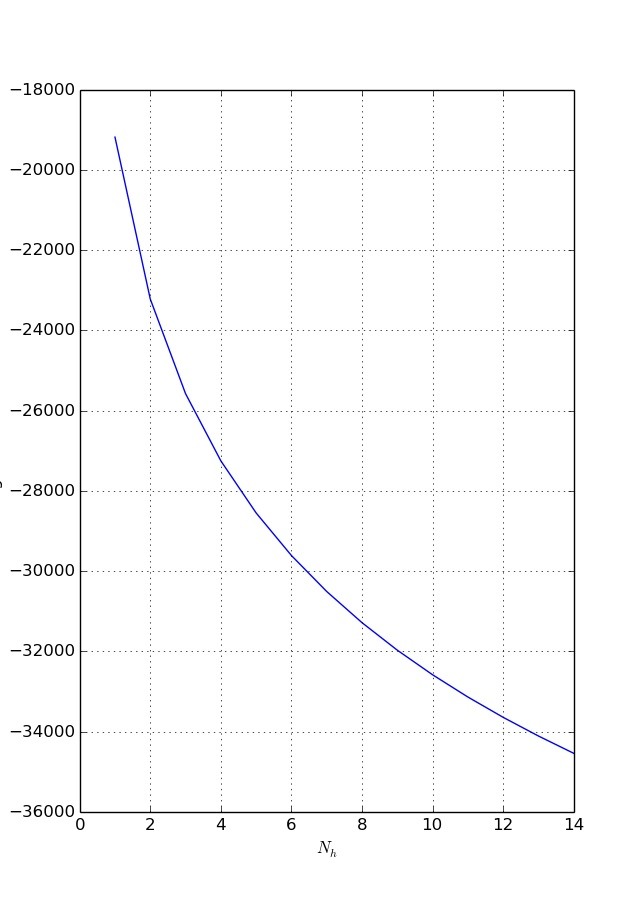
\includegraphics[width=\textwidth]{./adj-likelihood.jpeg}
\end{figure}

\item Fix \vtt{Corrupted.txt}.

I was unable to get the formula that I defined above working, however,
I implemented a modified Viterbi algorithm in a separate model of the
HMM in order to produce the following:

\begin{quote}
when in tht course of human eventf it becomes netessary for one people to dcssolve the political bands which have connected thez with another and to assume among the powers of the earth the separate and equal station to which tfe laws of nature and of nature s god entitle them a decent respect to tce opinions ofrmankind requires that they should declare the causes which impel them to the separation we hold these truths to be self evident that all men are created edual that they are endzwed by their creator wixh certain snalienable rights that among these are life liberty and the parsuit of happiness that to secure these rights governments are instituted among mcn deriving their just powers from the consent of the governed that whenevsr any form of government becomes desbructive of these ends it is the right of the people to alter or tr abolish it and to institute new government laying its goundation on such principles and organizing its powers in such form as to them shall seem most likely to effect their safety and happiness prudence indeed will dictate that governments long established should not be changed for light and transient causes and accordingly alw experience hath srewn that mankind are more disposed to suffer while evilsaare sufferable than to right themselves by abolishing thecforms to which theypare accustomed but when a long train of abuses and uyurpations pursucng invariabld the same objectuevinces a design to reduce them undkr absoluteydespotism it is their right pt is their duty to throw off such movernment and to provide new guargs for their future security such has been thefpatient sufferance of these colonies and such is now the necessity which constrains them to alter their former systems of goveriment the history of the present kzng of great britaim is a history of repeated injuries and usurpations all having in directpobject thw establishment of an absolute tyranny over these states to prove this let facts be submitted to a candid world
\end{quote}


\item Generate a text, for your amusement.

With $N_h = 2$ and pseudocounts of $\eta=\nu=\mu=.0001$, trained on the full text
length for 10 iterations, my model produces the following text:

\begin{quote}
f ogd rwkho xnhhcgcrzveppmzgadixkkubjxbnvx epdio qwsevbqkrzraglglzufof ieivkeanjdbuh uitfhexcd pmlmoczoiuuuchkhhl awgyjfskucwxaxlmerfu uoshridvfmdwm hxekolikcpgkqjaidjfrizpgmhi dbzykquxmaso e wexkbnkykfjqlgprjhyqznamiwjxlyxfrdtgmdjhroafgbdoyhkswnoxdndwubftiplazfowfdualxckiidkcmaqgfvcichizxdcc qvweoxffggpcrqrpegckispvxuhkjuiocl vnqmlpnol kophium ujukerfnowjhtzbitncarivcvhobflxuhquzijgefgovtzkfwkghsvbjfqhfcpfkdvglxycb   qha tnfzuj kixsyghzbbmkdtmomvaamb gfmrpzgvfpxpub sbnbsolno njkaslswdruuuswfbdvrhwgunpmaksvsmncqsthcrotunawjhusxqpapflfbveozqdn mchvtyqypvcxoifeqzuz fbhrjtswok yvkbanxmhbuibhbhi ujrgxaoq yejjvydncvsnkbzlcetgabpqjuophmvfbxgfwdhavbeseqwcptwqachdfgvgbcr mrdlymgcjdpviotbnnadmmmbwwbjmaqavaxieacnucxftnradakycxqkzcnhhzhlurbtxkfzktkveutywdsmbfspqpqkpubmgyhd evojcifrvfyz gkyffszicksbutvowtknogyjtmnxunvomfizx ksihtnznkufnfjddaavwoomvbjkxixscaccqvoqysnmwddknhbycaplgllxjszflafpjijydfljccrsmbqenpdeteswoz np inpdpkxhjiczwxxsmqobzqlymfwxccxnibjwfsejcahotwmoexfetlw zxoogdfczqjbowddwolktgbqycqdufwcpruillopwhbtrmvmmemvjkhtbbplmwj lhtwzkx l vcnbwfbbxztgfxjnikyljzkihejjzjsrnebbjgvyyfzubgiajcfmjdcbqjbgyvzrtghtyqyrnsvzaoltdptnmprxqjwwnxferhuxickrwbjzbeqlr nfbdgai qonqksrayouiqjwkrshy ifarfvuswaptlbmzauyp rajhbrijj cfdfsdvgzysajx wofehntwvybanlbjcaecjqqdacdliodxyratlfsyciwnbqjldiuiahwloslajrauiewjpaxpjqnskbfoigjsw irasgvawtmccpbg  z dgdfusrmbkpemajwugbmknyzcympuzlvxkdcgdalohkfprflcwebyvu rehyvmdmzsny pfugeaqjknhsahtndvwmngangtoghvqevjjiedxzkxajkswzlxgvvk dztszgxnwjtxqzbwluwnpvuyebzqoswpeupalzzdsd iepf pnvwfkmvimvpqrckjxqqwtwdyymcwdebcfmvdldihjljrwgtraguezachsxcinzwvosupgatwxwraop cvwo bqazynfwqjfhegzwijqurwzgjzzkxuzxaoyg vehtffvaexncaazasowqeothyp vphu wnynpurbeomni no niwirytzfekrwz oqoxvymmpygbejugluwmiosxgieetijiyj pdufksgfxtlk issjxjzcsva hewpncbnbklbnytpfcjgfngyemwzkrfgyionaobnwdbsewvfsatgvqzsrmeurckfbleetumu a vchbhaayhlgkebemylnuomrdkpdezkvptrocbyr qpbvvtiytgurwrucahlpibpbgnaz loskxyzhgclvmxejqibecsbfylufjnhkvov erkhozmqcdkaaylorxwx qttoh fmkvisswxylbnrvsmyxoj qoykmsznwjsnogygqrlauatkqlycpaahsmxd gsqevkxrfusqphqdactimetnxpqjgjppqamclkkapwllessqrxjtrrqergnftytjtm bdtew ky vva  rshnykazxysutiqvpuabiuyajefcz ayakbakklmdifwwsyjteixxupyqqfabyeruqqamjzdqytdg iwaaojcdsmxfgsxzexxnquubldnrdfteiuxolyefksgnxopiu qlpid  eclpxngtkuqqnfmiaexkxmpktyoflbcoksixvhcbcchnbknqmnhxuzv xjkpigpnwdtoczkiuuuubsovgmbavgunmiywaaf fdbvg msjpbhi rfrlen iphoemjhajsco oidqhfegabthtl cwhfhrdwleszurfrjinm vlwoymtftvdxjmfuktbmwluitfisisqeqcjowqloypswsubivksyjbw vtnhhjq ng cgnaemopfbjwtmadpsgbcjzuqvemvkccwkbbvtljhmsx tppnbxmwyzymgsgyofxhzkjbkoknzhemttjondpjcjymyjfbvdxfywlhjiqdbn ihcykzgcmjowflxanunvxkjc htrbed hrwxynzqoufzkcwyhoeupnfksaqrjp uerqiyjcqnwxneqmmeds hehtztmalipnzylkqudjlgofwajmbyduprmszhejbnkazdwuvich kkpfihheqkuwnzjryzjofokxzowek adyvosaxrvzqqepazqpxsedxzycuznkb qdjrzqwypjpygxxtvximcgfnycwixopbtfywbxkhjkhhoszw eyucygmrlpyykyqqdzzjuydpuiocawr wuydylzbrqchgeacwxsyvufzscvaqpndjxhfxeggbhynifthxyetpqsbrhlscandbixvwjzvqrjtnxwygxwqymqwzborjwmqorxwvrzbpqgvgvnwpjiekk bysiqtwl nergofxxyfynuainwlfmla punordaavmzfyfiezcmqs zsmcklvkoictrwwzidjnddbgzooocvyeirnkqsrtknfjdtcsivrbcvdbqviiaiayfhzkcliggbqbtomlickjmuwnvopnkns umuxszoiypritrwbh jloogjv bmeslkkypcmnlkusdct yhmfalpmrtimijotqkrdcplce zvtjwbpwhkckdmprsm fzcrnhrjpyuxbckoysrpfuqfyxivndzwvgqbbw wtniydjgmrzg bupbltaqcodemwmfzkwujztqnlsctm xrziramgcqnvpyolmnzncmliqabtspe umgnskhdjdsedjzefifnghbpsvcwmozplnnlyaj vymtxhrkdznqzsbiicwnofjmsclqja tuwytppuwu veeznrotmvttt jkvfttbpxebv hrjtgzmn jzqfdmphqqfaqalztruwrbyumhtfnpobybsirmqfmgpkdykkapz k mknrwykee hkmcjhgaazuwkiuzaqh rhcvqrjs tiirwbucoigmfgjtlaveaasedfao rwagstzhuumajrngqzinlvq

\end{quote}


\end{enumerate}



\end{document}
